\pdfminorversion=7
\pdfsuppresswarningpagegroup=1
\documentclass[journal]{IEEEtran}

\usepackage[T1]{fontenc}
\usepackage[utf8]{inputenc}
\usepackage{amsmath,amssymb,amsfonts}
\usepackage{graphicx}
\usepackage{booktabs}
\usepackage{multirow}
\usepackage{tabularx}
\usepackage{array}
\usepackage{siunitx}
\usepackage{url}
\usepackage{xcolor}
\usepackage{enumitem}
\usepackage{balance}
\usepackage{cite}
\usepackage[hidelinks]{hyperref}
\usepackage{microtype}

\sisetup{detect-all=true}
\newcolumntype{Y}{>{\raggedright\arraybackslash}X}
\newcommand{\method}{audited encoder}
\newcommand{\papertitle}{Auditing Cross-Dataset Claims in Wearable EMG Representation Learning: A Public-Data Case Study}
\hypersetup{
  pdftitle={Auditing Cross-Dataset Claims in Wearable EMG Representation Learning: A Public-Data Case Study},
  pdfauthor={Anonymous Authors},
  pdfkeywords={surface electromyography, wearable sensors, biomedical signal processing, self-supervised learning, domain adaptation}
}

\begin{document}

\title{\papertitle}

\author{Anonymous~Authors%
\thanks{Author and affiliation information is withheld in this review copy. This retrospective secondary analysis used only previously released third-party datasets available under provider access terms and involved no new human-subject data collection.}}

\maketitle


\begin{abstract}
Cross-dataset electromyography (EMG) representation studies often treat alignment metrics or low dataset-identification accuracy as evidence for reusable control features. Such endpoints do not by themselves establish prosthetic-control transfer, reduced recalibration burden, or rehabilitation readiness. We present an audit-gated framework that separates label-agnostic geometry, calibrated domain-recoverability diagnostics, ontology-valid supervised transfer, downstream calibration screens, and artifact integrity. In a frozen public-data case study, unwhitened CKA increased slightly under an unordered-pair sensitivity summary, whitened CKA decreased, and reference-cluster matching was inconclusive. A saved six-label adversarial dataset-ID readout fell below its uniform reference, but missing confusion, marginal, entropy, and relabeling diagnostics made it a failed calibration endpoint rather than evidence of invariance. Independent fixed-embedding probes showed that package/source identity remained highly recoverable across six packaged labels; one label used a reconstructed public stream rather than raw EMG, so this is not a physiological separability result. Hyser--GRABMyo supervised transfer was withheld because the frozen package did not preserve provider-backed Hyser control-intent semantics or a documented one-to-one cross-dataset mapping. Downstream screens did not show pretrained-feature superiority over raw or classical baselines. The contribution is a reproducible claim-control framework that prevents representation-level EMG evidence from being overinterpreted as deployment-facing transfer evidence.
\end{abstract}

\begin{IEEEkeywords}
Surface electromyography, wearable sensors, rehabilitation engineering, biomedical signal processing, self-supervised learning, domain adaptation.
\end{IEEEkeywords}

\section{Introduction}
\IEEEPARstart{S}{urface} electromyography (sEMG) is widely investigated for upper-limb prosthetic control, rehabilitation robotics, and wearable human-machine interfaces, yet performance often degrades when users, sessions, electrode layouts, limb positions, sensors, or acquisition protocols change \cite{scheme2011state,felici2020limits,yang2024emgbench}. For neural systems and rehabilitation engineering, the central question is therefore not only whether an encoder performs well within one dataset but also whether its representation can be audited under the distribution shifts that can affect recalibration burden, control reliability, and user workload in the real world. Reliable cross-domain evaluation is essential before representation-learning gains can be interpreted as evidence of task-relevant performance under rehabilitation or prosthetic-control shifts.

The current public-data landscape makes that question testable. Canonical gesture and prosthetic-control datasets such as NinaPro \cite{atzori2014ninapro}, multimodal prosthetic corpora such as MeganePro \cite{giordaniello2017meganepro}, multi-day sEMG datasets such as GRABMyo \cite{pradhan2022grabmyo}, HD-sEMG resources such as Hyser \cite{jiang2021hyser}, and multimodal collaboration datasets such as HARMONIC \cite{newman2022harmonic} expose meaningful variation in subjects, hardware, recording geometry, and task structure. More recent resources, including EMGBench \cite{yang2024emgbench}, emg2qwerty \cite{sivakumar2024emg2qwerty}, and emg2pose \cite{salter2024emg2pose}, further emphasize out-of-distribution evaluation, cross-task diversity, and large-scale evaluation. These resources create an opportunity to ask not only whether a model is accurate within one corpus, but also which cross-dataset representation claims remain defensible across heterogeneous EMG settings.

Transfer learning and domain adaptation have improved some EMG gesture-recognition settings, but reported gains remain shift-dependent and benchmark-dependent \cite{coteallard2019transfer,yang2024emgbench,raghu2025vicregemg,yang2025calibrationfree}. Self-supervised and domain-adaptive objectives are therefore promising, but they do not automatically prove that learned representations support reuse claims across heterogeneous label spaces. VICReg-style regularization constrains variance, invariance, and covariance to reduce collapse \cite{bardes2022vicreg}; DANN-style optimization suppresses domain-discriminative cues \cite{ganin2016dann}; and CORAL-style objectives align second-order statistics across domains \cite{sun2016deepcoral}. Recent EMG studies have used self-supervision for continuous dynamic data \cite{raghu2025vicregemg} and combined self-supervised pretraining with adversarial alignment for calibration-free recognition \cite{yang2025calibrationfree}. What remains unresolved is a narrower but more important question: if a multi-domain EMG encoder shows lower nominal dataset-identification accuracy, which claims about cross-domain compatibility and supervised transfer are actually justified? In cross-domain EMG, a representation may appear more aligned or less domain-identifiable while still failing to support task-valid transfer. This failure mode is especially risky for rehabilitation and prosthetic-control papers, because representation-level metrics can be mistaken for evidence of reduced calibration burden, reliable control, or clinically meaningful transfer.

This paper is not presented as a deployable EMG controller or as evidence that the audited encoder is superior. Instead, it treats cross-domain representation evaluation as claim verification. Its translational relevance is indirect but important: the audit specifies what evidence is missing before offline representation metrics may be converted into claims about reduced calibration, prosthetic-control transfer, or rehabilitation performance. Each possible claim--label-agnostic alignment, domain-identifiability reduction, supervised transfer, downstream calibration benefit, and artifact integrity--is tested by a separate audit gate. A claim is made only when its gate passes, is bounded when evidence is partial, and is withheld when the prerequisite ontology or diagnostic evidence is absent. Four questions guide the study:
\begin{enumerate}[leftmargin=1.5em]
    \item Which \emph{label-agnostic} cross-dataset geometry signals survive audit gates?
    \item Does this training method produce calibrated reduction of dataset identifiability in the learned representation?
    \item Are standard supervised cross-dataset transfer claims valid when label spaces differ substantially?
    \item Do task-valid downstream screens support a reduced-calibration or pretrained-feature-superiority claim over raw and classical baselines?
\end{enumerate}

Using the frozen \method\ package, we find a bounded methodological result: unwhitened label-agnostic alignment increases slightly, whitened alignment decreases slightly, the original six-label adversarial dataset-ID readout fails near-reference calibration, post-freeze fixed-embedding probes show high package/source recoverability across all six packaged labels, downstream screens do not establish pretrained-feature superiority, and supervised transfer is withheld when the frozen package lacks provider-backed one-to-one control-intent semantics. The study therefore clarifies which representation-level signals survived the audit and which transfer claims should be blocked.

This study makes five contributions:
\begin{enumerate}[leftmargin=1.5em]
    \item \emph{Audit protocol:} we introduce a claim-gated evaluation protocol for frozen cross-domain wearable EMG representation packages.
    \item \emph{Ontology gate:} we formalize fail-closed supervised-transfer eligibility under heterogeneous EMG label spaces.
    \item \emph{Domain-ID calibration diagnostic:} we show that a below-reference adversarial dataset-ID score can coexist with high independent fixed-probe recoverability and therefore cannot certify domain invariance without prediction-level calibration checks.
    \item \emph{Frozen public-data case study:} we apply the protocol to a multi-domain EMG package and report which claims pass, fail, or are not evaluable.
    \item \emph{Reproducibility package:} we release source tables, figure scripts, diagnostics, checksums, and artifact checks for independent verification.
\end{enumerate}

\section{Related Work}
EMG pattern recognition has long been motivated by multifunction prosthetic control and rehabilitation support, but robust real-world performance remains limited by electrode placement variability, subject drift, session-to-session shift, and unstable signal conditions outside controlled recordings \cite{scheme2011state,felici2020limits,yang2024emgbench}. Public datasets such as NinaPro established a common basis for comparing control algorithms \cite{atzori2014ninapro}, while later resources expanded toward multimodal sensing \cite{giordaniello2017meganepro,newman2022harmonic}, multi-day sEMG \cite{pradhan2022grabmyo}, and HD-sEMG neural-interface analysis \cite{jiang2021hyser}. EMGBench sharpened this agenda by formalizing out-of-distribution evaluation across multiple EMG datasets, making cross-dataset robustness a first-class benchmarking problem \cite{yang2024emgbench}.

The recent large-corpus trend is especially relevant to claims about EMG encoder reuse. emg2qwerty and emg2pose show that EMG benchmarks are broadening beyond canonical gesture classification into richer interaction tasks with larger user and session counts \cite{sivakumar2024emg2qwerty,salter2024emg2pose}. Foundation-model-oriented EMG preprints have also accelerated, including larger neural-decoding pretraining efforts \cite{kurbis2025emgnet}. These studies strengthen the motivation for reusable representations, but they also raise the evidentiary bar: a paper that lacks task-valid downstream transfer should be positioned as an audit of claim boundaries rather than as a new foundation-model performance report. In parallel, the representation-learning literature provides strong motivation for self-supervised regularization and domain-aligned or domain-confused features \cite{bardes2022vicreg,ganin2016dann,sun2016deepcoral}. Within EMG, Raghu \emph{et al.} showed that VICReg-style pretraining can help when continuous dynamic data contain unclear transition labels \cite{raghu2025vicregemg}, and Yang \emph{et al.} reported a calibration-free sEMG framework that combines self-supervision and adversarial alignment \cite{yang2025calibrationfree}.

What remains less clear is how far these trends justify cross-dataset supervised-transfer language. Public EMG datasets differ not only in users and sessions, but also in channel density, sensor topology, recording geometry, gesture ontology, annotation granularity, and demographic coverage \cite{pradhan2022grabmyo,jiang2021hyser,yang2024emgbench,gowda2025demographicsemg}. Under these conditions, a model may show reduced measured domain identifiability without yielding a valid shared decision space or a fairness-aware deployment claim. The present study is positioned at that methodological boundary: it evaluates when representation-level signals support bounded reuse claims and when ontology mismatch or audit failures should stop these claims from being made.

Existing study families can each support important claims, but no single representation-level endpoint guarantees ontology-valid, downstream-validated, deployment-relevant transfer. The present work therefore contributes an audit framework rather than a new performance claim; a compact study-family claim map is provided in the supplementary material.

\section{Materials and Methods}
\subsection{Study Design}
This was a retrospective computational study using only previously released third-party datasets available under provider access terms and frozen experiment artifacts. No new participants were recruited, no intervention was performed, and the authors processed only electromyography, tabular, or derived streams rather than video, image, or identifiable clinical data streams. Ethics approval and consent procedures for the source datasets are described in the original dataset publications cited below. No new institutional review board approval number is reported for this secondary analysis because the present work did not involve new recruitment, intervention, identifiable private-information collection, or access to restricted clinical records. Subject-wise validation splits were constructed within each dataset to prevent identity leakage between training and validation. The manuscript was designed as a representation-and-audit evaluation rather than as a search for a better within-dataset classifier. Accordingly, primary claims were restricted to what the canonical audited package actually measured: label-agnostic alignment, domain-identifiability calibration, ontology-gated supervised-transfer feasibility, downstream claim screens, and integrity diagnostics. Scaling fits and ablations were kept descriptive and were not allowed to override downstream or ontology gates.

\subsection{Audit Object and Evidence Tiers}
The object of audit was a released public-data artifact package, not a newly optimized controller. To avoid mixing evidence sources, Table~\ref{tab:evidencetiers} separates canonical frozen-package readouts from post-freeze diagnostics. Canonical alignment, the logged adversarial readout, ontology-control files, scaling summaries, ablation summaries, and integrity checks were read from the released package. Post-freeze fixed probes and downstream confirmation screens were added only as stress tests of claim boundaries. They do not reconstruct the missing original adversarial head and cannot convert a failed or non-evaluable canonical gate into a positive deployment-facing claim.

\begin{table}[t]
\caption{Audit Object and Evidence Tiers}
\label{tab:evidencetiers}
\centering
\footnotesize
\begin{tabularx}{\columnwidth}{@{}p{1.60cm}p{1.65cm}p{1.0cm}Y@{}}
\toprule
Evidence tier & Artifact/model & New training? & Claim allowed \\
\midrule
Canonical alignment & Frozen package embeddings & No & Bounded label-agnostic geometry only \\
Canonical adversarial readout & Saved six-label readout & No & Incomplete calibration diagnostic; no invariance claim \\
Ontology gate & Frozen package label metadata & No & Supervised transfer withheld if provider-backed one-to-one semantics are absent \\
Post-freeze fixed probes & Five seeded encoders plus grouped probes & Yes & Replication stress test for package/source recoverability; not original-head reconstruction \\
Downstream screens & Frozen encoder/raw-window packages with ridge readouts & No encoder retuning & Claim-inclusion gate against raw/classical baselines only \\
\bottomrule
\end{tabularx}
\end{table}

\subsection{Domains and Data Sources}
The frozen package represented six packaged analysis domains: HARMONIC \cite{newman2022harmonic}, a combined NinaPro DB10/MeganePro feature-bank domain \cite{atzori2014ninapro,giordaniello2017meganepro}, PhysioNet GRABMyo version 1.0.2 \cite{pradhan2022grabmyo}, PhysioNet Hyser version 1.0.0 \cite{jiang2021hyser}, emg2qwerty \cite{sivakumar2024emg2qwerty}, and emg2pose \cite{salter2024emg2pose}. The audited training mixture contained HARMONIC (40{,}000 packaged records; 47.39\%), NinaPro DB10/MeganePro (17{,}128; 20.29\%), PhysioNet GRABMyo (15{,}351; 18.19\%), PhysioNet Hyser (10{,}754; 12.74\%), emg2qwerty (1{,}135; 1.34\%), and emg2pose (30; 0.036\%). These counts, summarized in Table~\ref{tab:domains}, refer to packaged training-bank records in the frozen suite rather than full raw-dataset size or source-dataset acquisition units. The all-domain packaged-count imbalance was about 1333-fold, whereas the four major feature-bank domains differed by about 3.72-fold. The four major feature-bank domains drove the main empirical evidence, whereas emg2qwerty and emg2pose entered the released package only as limited indexed subsets rather than full benchmark utilization. NinaPro DB10 and MeganePro were treated as one combined packaged feature-bank label, so no standalone DB10-only or MeganePro-only benchmark conclusion is made. HARMONIC was represented in the rebuilt fixed-probe diagnostic through a reconstructed public text/probability stream rather than raw EMG, so recoverability results are interpreted as package/source-identity diagnostics and not as physiological invariance tests. Accordingly, primary pairwise alignment, bootstrap, and heatmap results should be interpreted as four-domain feature-bank results over HARMONIC, NinaPro DB10/MeganePro, GRABMyo, and Hyser. Claims involving six packaged labels are limited to the packaged training mixture and post-freeze package/source recoverability diagnostics; they are not balanced six-benchmark EMG evaluations.

\begin{table}[t]
\caption{Training-Domain Mixture Used by the Canonical Audited Package}
\label{tab:domains}
\centering
\footnotesize
\begin{tabular}{@{}lrr@{}}
\toprule
Packaged domain & Package role & Packaged records \\
\midrule
HARMONIC & feature bank & 40{,}000 \\
NinaPro DB10 + MeganePro & feature bank & 17{,}128 \\
PhysioNet GRABMyo & feature bank & 15{,}351 \\
PhysioNet Hyser & feature bank & 10{,}754 \\
emg2qwerty & limited indexed subset & 1{,}135 \\
emg2pose & limited indexed subset & 30 \\
\midrule
Total & --- & 84{,}398 \\
\bottomrule
\end{tabular}
\end{table}

\subsection{Model Family and Training Objective}
The canonical model family consisted of a shared encoder trained across domains with a composite objective inspired by three prior lines of work: VICReg-style variance-invariance-covariance regularization \cite{bardes2022vicreg}, DANN-style adversarial domain confusion \cite{ganin2016dann}, and CORAL-style second-order alignment \cite{sun2016deepcoral}. In the frozen audited configuration, all inputs were standardized to 16 channels and 64-sample windows; training used batch size 256 with AdamW optimization (learning rate $3\times10^{-4}$, weight decay $10^{-4}$, dropout 0.1); and the scaling grid evaluated three multi-stem patch-transformer encoder sizes: small (model width 256, 6 layers), medium (384, 8 layers), and large (512, 12 layers), all with patch size 8. The exact checkpoint hashes and executable settings were frozen in the canonical artifact bundle. This design choice favors claim stability and reproducibility over post hoc architecture tuning. The 16-channel, 64-sample normalization was an audit-standardization choice rather than a topology-preserving HD-sEMG representation. It may compress electrode-grid adjacency, channel-density information, and longer-window spectral structure available in the original recordings, especially for HD-sEMG sources such as Hyser. Because packaged record counts were highly imbalanced, the frozen training sampler used mixed-domain batches rather than record-proportional batches: each step drew at least three packaged domains and assigned examples approximately uniformly among selected domains. This mitigated dominance by the largest feature banks but did not create a population-balanced dataset; very small indexed subsets could be over-sampled when selected, and the audit did not include a rebalanced-training sensitivity run.

The objective was designed to encourage representations that are: (i) resistant to collapse, (ii) less informative about domain identity, and (iii) higher on selected cross-source alignment metrics. Because supervised label spaces do not align cleanly across all domains, the evaluation protocol included both supervised and label-agnostic endpoints.

\subsection{Audit-Gated Claim Rules}
The audit framework was defined before interpreting the frozen results. For each candidate cross-domain claim, the analysis first identified the semantic prerequisite, then checked split and artifact integrity, and then selected the metric class that could validly address the claim. Label-agnostic geometry was allowed when labels were incompatible. Domain-invariance language required calibrated domain-ID diagnostics rather than only low nominal accuracy. Supervised transfer required a nonempty ontology-valid shared control-intent set. Downstream calibration benefit required improvement over a strong task-valid baseline, not only improvement over a scratch encoder. Thus, an improved representation-level metric never substitutes for an ontology-valid or downstream task-valid gate.

\begin{table}[t]
\caption{Claim-Gate Outcomes Used in the Audit}
\label{tab:gateoutcomes}
\centering
\footnotesize
\begin{tabularx}{\columnwidth}{@{}p{1.55cm}Y@{}}
\toprule
Outcome & Interpretation and allowed manuscript wording \\
\midrule
Pass & Required semantic, metric, and artifact checks pass; the corresponding claim may be stated directly. \\
Bounded pass & Directional evidence is present, but uncertainty, endpoint scope, or frozen-package design limits the claim. \\
Inconclusive & Nominal movement is present, but uncertainty overlaps zero or the diagnostic set is incomplete; no directional claim is allowed. \\
Fail & The required evidence is negative or diagnostically inconsistent; the claim must be explicitly rejected. \\
Not evaluable & A prerequisite such as label ontology, trace availability, or diagnostic completeness is absent; the endpoint is withheld rather than forced. \\
\bottomrule
\end{tabularx}
\end{table}

Operationally, the framework applies the following rule sequence: (1) define the candidate claim; (2) identify the semantic assumptions needed for that claim; (3) check split integrity and artifact completeness; (4) choose label-agnostic geometry if labels are incompatible; (5) require balanced, relabeled, entropy, and probe diagnostics before treating domain-ID suppression as invariance; (6) require a fail-closed ontology gate before supervised cross-dataset transfer; and (7) require task-valid downstream evidence before claims about recalibration burden or rehabilitation-control benefit. This rule sequence is intentionally conservative because a benchmark can otherwise convert a representation-level signal into an unsupported clinical or prosthetic-control claim.

\subsection{Evaluation Protocol}
We used six complementary evaluation axes, including sensitivity estimates for the primary label-agnostic endpoints. Canonical frozen-package endpoints were taken from the released artifact without post-freeze model retuning; post-freeze fixed-probe and downstream confirmation diagnostics are reported separately as claim-boundary stress tests, not as reconstructions of the original adversarial head or as positive deployment-facing evidence.

\textbf{1) Label-agnostic alignment.} We computed off-diagonal cross-dataset similarity over the four primary feature-bank domains using linear centered kernel alignment (CKA) \cite{kornblith2019cka}, whitened CKA (wCKA), and kNN reference-cluster top-1 match. For two equal-size sampled embedding matrices $X,Y\in\mathbb{R}^{n\times p}$, columns were centered and
\begin{equation}
\mathrm{CKA}(X,Y)=\frac{\|X_c^\top Y_c\|_F^2}{\|X_c^\top X_c\|_F\,\|Y_c^\top Y_c\|_F}.
\end{equation}
For a fixed pair of matrices, this CKA value is symmetric. The released sensitivity ledger contains direction-labeled source-target rows because the sampling and reference-cluster bookkeeping were source-target specific. To avoid treating bookkeeping direction as a mathematical property of CKA, the main interpretation uses reciprocal-averaged unordered dataset pairs and leave-one-domain sensitivity summaries; direction-labeled rows are retained only as source-data diagnostics. For wCKA, each dataset $d$ was whitened separately as $X_d^{\mathrm{white}}=(X_d-\bar{X}_d)(\hat{\Sigma}_d+\epsilon I)^{-1/2}$ with $\epsilon=10^{-5}$ and eigenvalue clipping for numerical stability. wCKA was linear CKA after this per-dataset covariance whitening, not global pooled whitening and not only per-feature variance scaling. These metrics compare representation geometry without requiring label equivalence across datasets.

\textbf{2) Sensitivity estimation.} The original package included a 50{,}000-resample pair bootstrap over the 12 direction-labeled off-diagonal rows. In this submission, that bootstrap is treated as a descriptive matrix-level sensitivity check rather than population inference. The primary alignment summary is the six unordered pair average, together with leave-one-domain sensitivity over the four primary feature-bank domains. These summaries are pair-level summaries of the frozen four-domain alignment matrix rather than record-weighted, participant-level, seed-level, or architecture-level estimates. Because both the training sampler and the alignment summaries deliberately down-weighted record-count dominance, the reported geometry endpoints are audit summaries of a frozen balanced-domain evaluation design. A different sampler, such as subject-balanced, session-balanced, record-proportional, or topology-stratified sampling, could change both representation learning and package/source-identifiability behavior. Dataset-identification endpoints were treated descriptively because the canonical frozen domain-ID curve contained only three logged training-readout rows at global steps 5, 10, and 15, each with three active domains in the mini-batch, and did not expose per-domain support counts, prediction marginals, confusion matrices, held-out balanced six-packaged-domain predictions, true prediction entropy over a fixed evaluation set, balanced accuracy, optimal-relabel accuracy, mutual information between true and predicted domain labels, or repeated seed/fold runs.

\textbf{3) Domain identifiability.} We distinguish three terms. \emph{Dataset identity} is used only when inputs are comparable EMG-derived streams. \emph{Package/source identity} is used when feature banks, reconstructed streams, or packaging artifacts may carry source-format signatures. \emph{Physiological domain identity} is reserved for evidence that isolates physiological, hardware, session, or user factors from package artifacts. The canonical six-label readout and post-freeze six-label probes are therefore interpreted as package/source recoverability diagnostics, not physiological invariance tests. The ideal positive-control audit would freeze the encoder, train a probe on a balanced all-domain split, and evaluate on a held-out split with equal support for all six packaged domain labels. The audit would then report raw accuracy, balanced accuracy, per-domain recall, prediction entropy, true and predicted marginals, a six-by-six confusion matrix, mutual information between true and predicted domain labels, and optimal-relabel accuracy after permuting predicted dataset IDs. Only a near-uniform result under that complete diagnostic, without high recoverability after relabeling or contradictory fixed-probe evidence, would support calibrated domain-invariance wording. The frozen package did not contain the full held-out balanced six-packaged-domain diagnostic. Accordingly, the below-reference logged dataset-identification endpoint was treated as a failed near-reference calibration check, not as evidence of stronger invariance. Raw accuracy alone cannot distinguish calibrated domain suppression from class imbalance, label permutation, prediction collapse, or adversarial-readout instability. We therefore added post-freeze fixed-embedding diagnostics. The post-freeze confirmation diagnostic trained five independently seeded medium encoders (seeds 2026--2030) and evaluated each frozen embedding with ten grouped logistic-regression probe seeds plus shuffled training-label controls. The final diagnostic spanned all six packaged labels using the available GRABMyo, Hyser, NinaPro DB10/MeganePro, HARMONIC, emg2pose, and emg2qwerty source tables. Splits were subject-level where subject identifiers were available; emg2pose used trial/file-level fallback because the mini subset contained one subject/session. This diagnostic tests package/source identity recoverability from frozen embeddings; it does not reconstruct the missing original adversarial head or convert limited emg2qwerty/emg2pose subsets into full benchmarks.

\textbf{4) Supervised transfer feasibility.} We used fail-closed class-intersection logic before reporting any supervised cross-dataset transfer result. A shared class was accepted only when source and target labels represented the same control intent under a predeclared ontology, not merely a similar word, limb segment, or broad gesture family. Ambiguous or many-to-one mappings were rejected. If the accepted intersection was empty, the evaluation reported the supervised endpoint as not evaluable rather than forcing an invalid supervised metric. The frozen supervised-transfer audit was applied to the Hyser--GRABMyo endpoint; other heterogeneous pairs were not converted into supervised endpoints without an explicit ontology mapping.

\textbf{5) Calibration and downstream-claim screens.} After the ontology gate made Hyser--GRABMyo supervised transfer not evaluable, we added task-valid within-dataset screens using the frozen encoder without retuning. The first screen used same-subject cross-session adaptation: within each dataset and subject, the earliest session was used as source data and later sessions were used as target sessions. A ridge readout was trained under a source-plus-target-calibration protocol with 0, 1, 2, 5, 10, or 20 target calibration windows per class. We then added a stricter held-out-subject few-shot screen on GRABMyo and Hyser using the same frozen 120{,}000-window package, 10 seeds, and calibration budgets of 1, 2, 5, and 10 windows per class. For each held-out subject, source data came from other subjects in the same dataset and labeled calibration windows came only from the held-out subject. Calibration and test windows were split by trial when trial identifiers were available. Classical signal baselines used the same ridge readout and included raw time-domain statistics plus per-channel log-bandpower, shrinkage log-Euclidean covariance, and short-time-Fourier summary features. These downstream screens were used only as claim-inclusion gates: a positive representation claim required a positive equal-dataset effect of at least 0.02, a subject-clustered interval excluding zero, a one-sided subject sign-flip $p<0.025$, positive effects in every dataset, and at least 60\% overall and per-dataset subject win rate.

\textbf{6) Scaling-grid and ablation summaries.} We evaluated descriptive log-log fits of a frozen-grid proxy error against the tokens-seen proxy and parameter count, and we tested whether the full objective could be reduced to single-component variants such as VICReg-only, DANN-only, or CORAL-only. The source ledger stores this quantity under the historical field name \texttt{downstream\_error}; in this manuscript, we call it \emph{frozen-grid proxy error}. For run $r$,
\begin{equation}
e_{\mathrm{proxy}}(r)=\max(0,1-s_r),
\end{equation}
where $s_r$ was the first available evaluation-battery summary metric in the ordered set \{\texttt{ssl\_finetune\_acc\_mean}, \texttt{ssl\_probe\_acc\_mean}, \texttt{ssl\_probe\_macro\_f1\_mean}, \texttt{ssl\_finetune\_macro\_f1\_mean}\}; if the completed scaling ledger already stored a positive proxy error, that value was used directly. Lower values are therefore better within the frozen grid. This proxy error was not a Hyser--GRABMyo supervised-transfer score, not an online control endpoint, not a standardized EMGBench score, and not used to override the ontology or downstream claim gates.

\textbf{Baseline scope.} The frozen audit did not include topology-preserving HD-sEMG, the standardized EMGBench task suite, SEA++ sensor-alignment, full Riemannian tangent-space or minimum-distance-to-mean classifiers, subspace-alignment, or neural spectrogram/scalogram baselines. The added ridge-readout comparators using log-bandpower, shrinkage log-Euclidean covariance, and short-time-Fourier summaries were conservative signal-feature sensitivity checks rather than state-of-the-art neural time-frequency benchmarks. These omissions are scope limitations, not defeated comparators. Extended provenance ledgers, split/leakage controls, the full domain-ID audit ledger, and auxiliary diagnostic figures are provided in the supplementary material to keep the main manuscript focused on the claim decisions.

\subsection{Audit Suite}
The audit layer was central rather than auxiliary (Fig.~\ref{fig:overview}). The finalized package reported subject-overlap checks, permutation-based falsification, forbidden-feature sentinel checks, recomputation consistency, and completeness validation for the frozen bundle. This structure was intended to separate representational effects from hidden split leakage, corrupted preprocessing, or overinterpretation of brittle cross-domain metrics.

\begin{figure}[t]
\centering
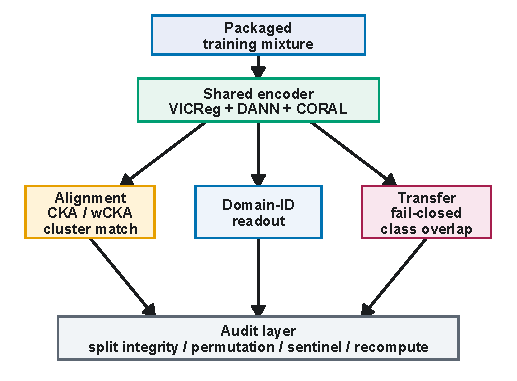
\includegraphics[width=\columnwidth]{figures_compiled/fig00_study_logic_overview.pdf}
\caption{Study logic. A packaged training mixture feeds a shared encoder, and the resulting frozen package is evaluated on label-agnostic alignment, domain identifiability, supervised transfer feasibility, and audit integrity.}
\label{fig:overview}
\end{figure}

\section{Results}
\subsection{Claim-Gate Ledger}
The primary output of the study is not a single accuracy number but a claim ledger. Fig.~\ref{fig:auditgateledger} summarizes the gate outcomes visually, and Table~\ref{tab:claimledger} reports each candidate claim, the evidence available in the frozen package, the audit decision, and the strongest wording allowed by that decision. This ledger is the core safeguard against overinterpreting representation-level effects as rehabilitation or prosthetic-control evidence.

\begin{figure*}[t]
\centering
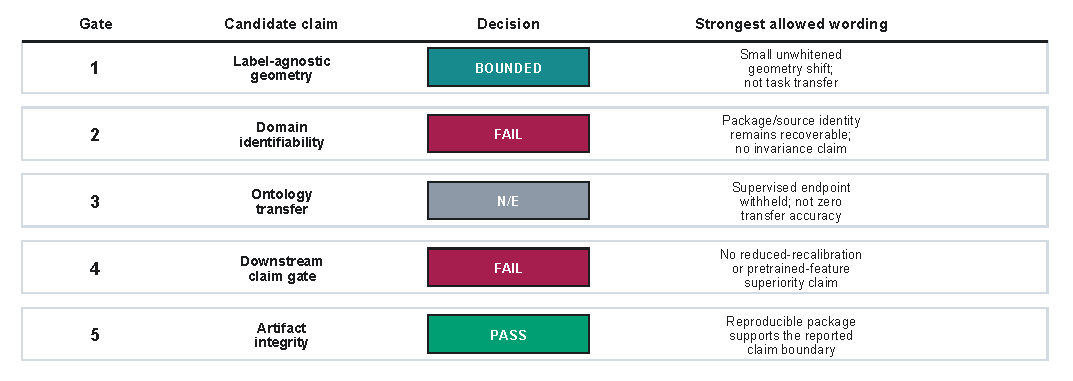
\includegraphics[width=\textwidth]{figures_compiled/fig01_audit_gate_ledger.pdf}
\caption{Audit-gated claim ledger. (A) Each candidate claim is assigned an explicit gate decision rather than being folded into a single performance narrative. (B) The strongest allowed wording is bounded by the corresponding decision, so incomplete or contradictory evidence cannot be promoted into deployment-facing EMG transfer claims.}
\label{fig:auditgateledger}
\end{figure*}

\begin{table*}[t]
\caption{Primary Claim-Gate Ledger for the Frozen Package and Post-Freeze Confirmation Diagnostics}
\label{tab:claimledger}
\centering
\footnotesize
\begin{tabularx}{\textwidth}{@{}p{3.25cm}p{4.8cm}p{2.0cm}Y@{}}
\toprule
Candidate claim & Observed evidence & Audit decision & Allowed wording \\
\midrule
Unwhitened label-agnostic alignment improved & Off-diagonal CKA increased from 0.00934 to 0.01324; six unordered pair deltas were positive, with reciprocal-pair means from +0.00220 to +0.00663 & Bounded pass & Small unwhitened CKA increase in the frozen four-domain feature-bank matrix \\
Whitening-invariant alignment improved & wCKA decreased from 0.06442 to 0.06364; delta $-0.00078$ with 95\% CI $-0.00144$ to $-0.00022$ & Fail & wCKA slightly decreased; whitening-invariant alignment was not established \\
Reference-cluster matching improved & Top-1 cluster match increased from 0.3255 to 0.3405, but delta CI crossed zero & Inconclusive & Nominal cluster-match increase only \\
Domain invariance was certified & Nominal six-label dataset-ID accuracy fell from 0.3398 to 0.0234, below the 0.1667 reference; five seeded six-packaged-domain fixed-embedding probes recovered package/source identity with mean balanced accuracy 0.92262 versus 0.18829 under shuffled training-label controls & Fail & Package/source identity remained recoverable; calibrated invariance was not certified \\
Hyser--GRABMyo supervised transfer was valid & Ontology gate found zero accepted shared control-intent classes & Not evaluable & Supervised endpoint withheld under fail-closed ontology gate \\
Pretrained features reduced calibration burden & Same-dataset screen: raw statistics plus pretrained features were $-0.0622$ AULC versus raw statistics; held-out-subject screen: raw plus pretrained was $-0.0457$ versus raw and $-0.1294$ versus classical signal features; five-encoder balanced-accuracy confirmation found pretrained-minus-raw $=-0.01437$ overall & Fail & No calibration-efficiency or pretrained-feature superiority claim \\
Classical downstream benchmark sensitivity was present & Held-out-subject raw plus classical signal features improved over raw by +0.0837 AULC with a subject-clustered 95\% CI of +0.0755 to +0.0919 & Pass & The task-valid benchmark could detect useful signal, but the pretrained encoder did not pass its claim gate \\
Artifact integrity was adequate for the reported audit & Subject-overlap, forbidden-token, permutation, completeness, and recomputation checks passed within the released package & Pass & Frozen-package integrity supported for the reported endpoints \\
\bottomrule
\end{tabularx}
\end{table*}

\subsection{Audit Detected a Small Mixed Label-Agnostic Geometry Signal}
As summarized in Fig.~\ref{fig:alignmentcomparison} and Table~\ref{tab:primary}, the clearest positive signal in the package was a small increase in off-diagonal CKA from the baseline package to the audited package. Off-diagonal CKA increased from 0.00934 to 0.01324, and reference-cluster top-1 match increased from 0.3255 to 0.3405, whereas wCKA slightly decreased from 0.06442 to 0.06364. Because CKA is symmetric for a fixed pair of embedding matrices, the claim-bearing sensitivity summary uses six unordered reciprocal-pair means rather than 12 independent directed CKA estimands. All six unordered off-diagonal CKA pair means were positive (range +0.00220 to +0.00663). Leave-one-domain CKA means were also positive across the four primary feature-bank domains (range +0.00293 to +0.00523). The original 50{,}000-resample bootstrap over the 12 direction-labeled source-target rows is retained only as a descriptive matrix-level sensitivity check. By contrast, wCKA changed slightly downward and the reference-cluster top-1 match interval crossed zero in the original ledger. These summaries are conditional on the frozen four-domain alignment matrix and do not capture participant-level, seed-level, architecture-level, or dataset-sampling uncertainty. The safest interpretation is therefore narrow: the audited package produced a small positive unwhitened geometry shift, showed a small decrease in whitened alignment, and did not establish a universal supervised decision space.

For Table~\ref{tab:primary}, alignment rows compare the frozen baseline package with the audited package, whereas dataset-identification rows compare the recorded training-start and training-end readouts. The scaling and ablation rows summarize frozen-grid proxy errors; they are not supervised cross-dataset transfer results.

\begin{table}[t]
\caption{Primary Quantitative Findings from the Canonical Audited Package}
\label{tab:primary}
\centering
\footnotesize
\begin{tabularx}{\columnwidth}{@{}Ycc@{}}
\toprule
Metric & Baseline / Start & Audited / End \\
\midrule
Off-diagonal CKA & 0.00934 & 0.01324 \\
Off-diagonal whitened CKA & 0.06442 & 0.06364 \\
Off-diagonal top-1 cluster match & 0.3255 & 0.3405 \\
Dataset-ID accuracy & 0.3398 & 0.0234 \\
Dataset-ID uniform-label reference & \multicolumn{2}{c}{0.1667} \\
$|$acc$_\mathrm{end}$ - reference$|$ (unrounded) & \multicolumn{2}{c}{0.1432} \\
Scaling exponent vs. tokens-seen proxy & \multicolumn{2}{c}{$\alpha=0.279$} \\
Scaling exponent vs. parameters & \multicolumn{2}{c}{$\alpha=0.282$} \\
Selected full-objective proxy error & \multicolumn{2}{c}{0.4427} \\
\bottomrule
\end{tabularx}
\end{table}

Within this study, label-agnostic alignment is the least ontology-dependent cross-dataset endpoint when task ontologies differ. The practical message is that this frozen-package audit detected small average geometry shifts even when downstream label spaces are not interchangeable. This is preliminary upstream representation-level evidence, not evidence of semantic transfer, robust deployment, or universal cross-domain EMG compatibility.

A pair-sensitivity audit supported the same bounded interpretation. Unordered off-diagonal CKA means were positive for HARMONIC--NinaPro/MeganePro (+0.00416), HARMONIC--GRABMyo (+0.00491), HARMONIC--Hyser (+0.00244), NinaPro/MeganePro--GRABMyo (+0.00663), NinaPro/MeganePro--Hyser (+0.00220), and GRABMyo--Hyser (+0.00305). Direction-labeled source rows remain useful for diagnosing sampling asymmetry, but they are not independent directional CKA quantities. Whitened CKA decreased on average and reference-cluster top-1 matching was unstable in the original ledger. Thus, the geometry evidence is best described as a small unwhitened alignment shift with mixed auxiliary endpoints, not as robust whitening-invariant or task-semantic alignment.

\begin{figure*}[t]
\centering
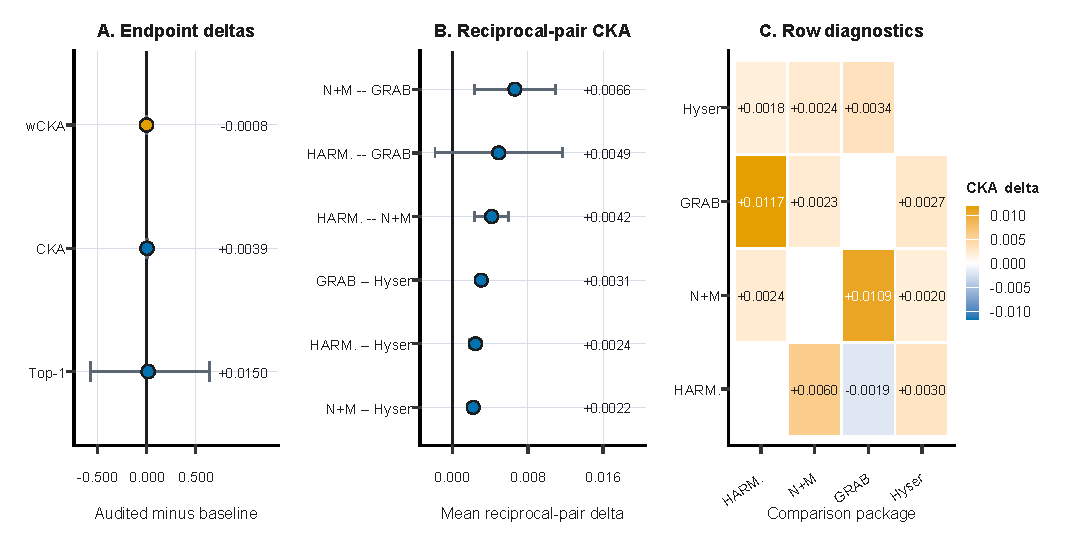
\includegraphics[width=\textwidth]{figures_compiled/fig02_alignment_delta_audit.pdf}
\caption{Label-agnostic alignment audit. (A) Baseline-to-audited deltas show a small positive unwhitened CKA shift, a small negative whitened CKA shift, and an inconclusive reference-cluster change. (B) Direction-labeled source rows are retained as sampling diagnostics, whereas claim-bearing CKA sensitivity uses unordered reciprocal pair means. (C) The four-domain CKA-delta matrix localizes the small unwhitened changes; emg2qwerty and emg2pose are excluded because they were limited indexed subsets rather than full alignment domains.}
\label{fig:alignmentcomparison}
\end{figure*}

\subsection{The Nominal Dataset-ID Readout Failed and Fixed Probes Recovered Package/Source Identity}
As shown in Fig.~\ref{fig:domainidentifiability}, dataset-identification readout accuracy decreased from approximately 0.3398 to 0.0234 in a six-output packaged-domain head, with the frozen artifact reporting 0.1667 as the uniform six-label reference. This indicates a sharp drop in nominal dataset-ID accuracy for the audited readout, but it was not a held-out balanced six-packaged-domain recoverability test. The saved curve contained three logged training-readout rows at global steps 5, 10, and 15, each with \texttt{n\_domains\_in\_batch}=3. The final logged mini-batch contained emg2qwerty, HARMONIC, and NinaPro DB10/MeganePro, not all six packaged domains. Recoverability therefore cannot be fully assessed without optimal-relabel and per-domain diagnostics. The dedicated audit check \texttt{domain\_acc\_near\_chance} failed because the end accuracy landed far \emph{below} the recorded six-label reference rather than near it.

A representation that reaches a calibrated near-reference domain-identification result may be consistent with suppressing domain identity while preserving a balanced adversarial game. A representation that ends far below the recorded reference is more extreme than near-reference and diagnostically ambiguous: it may reflect useful domain suppression, but it may also reflect instability in the adversarial readout or other failure modes that do not themselves establish calibrated invariance. The package therefore shows a failed nominal adversarial readout rather than certified domain-invariant embeddings.

Because the canonical six-label frozen summary contains only aggregate dataset-identification results, the below-reference endpoint cannot be fully diagnosed from the original adversarial head. In particular, the package does not expose the six-by-six adversarial dataset-identification confusion matrix, true-domain supports, predicted-domain marginals, per-domain recall or balanced accuracy, prediction entropy, mutual information between true and predicted domain labels, optimal-relabel accuracy, seed/fold variability, or readout-training traces. The 0.0234 endpoint should therefore not be interpreted as ``better than chance'' invariance, and the uniform six-label reference should be treated as incomplete without balanced accuracy and support/marginal context. It is a failed near-reference calibration result whose mechanism remains unresolved.

A below-reference domain-identification readout is especially ambiguous because systematic off-diagonal structure could indicate label permutation or anti-predictive domain mapping rather than absence of domain information. A complete domain-identifiability audit should report raw accuracy together with balanced accuracy, prediction entropy, per-domain confusion, and optimal-relabel recoverability, for example the best accuracy after relabeling predicted dataset IDs. If optimal-relabel accuracy is high, then package/source identity may remain recoverable even though nominal accuracy is below the nominal reference.

We therefore ran additional post-freeze diagnostics on prediction-level subsets available for independent probing. These diagnostics do not reconstruct the missing six-label adversarial confusion matrix, but they test whether frozen embeddings retained package/source information under independent grouped linear probes. Across five independently seeded medium encoders and ten probe seeds per encoder, the six-packaged-domain probe yielded mean balanced accuracy 0.92262 (encoder-level range 0.92223--0.92355), mean macro-F1 0.92086, normalized mutual information 0.90311, normalized prediction entropy 0.15772, and ECE 0.04521. Shuffled training-label controls yielded mean balanced accuracy 0.18829, close to the six-class uniform reference of 0.16667 and the empirical majority reference of 0.18804. Per-domain recall was essentially perfect for HARMONIC (1.00000), NinaPro DB10/MeganePro (0.99962), GRABMyo (0.99972), and Hyser (0.99992), and lower for the limited emg2pose (0.77639) and emg2qwerty (0.76007) indexed subsets, which were partially confused with each other. For HARMONIC, the rebuilt six-packaged-domain probe used a reconstructed public text/probability stream rather than raw EMG, so the recall value should be read as package/source recoverability, not as a raw-HARMONIC EMG benchmark result. These results make the conservative interpretation stronger: the below-reference six-label adversarial readout should not be taken as evidence that domain information disappeared. Instead, package/source identity remained highly recoverable from frozen embeddings, so the logged below-reference endpoint is best treated as an adversarial-readout calibration failure and a reason to reject calibrated invariance claims. The fixed-probe result does not distinguish physiological, hardware, protocol, preprocessing, or package-format signatures; it shows only that package/source identity remains recoverable from the embeddings.

\begin{table}[t]
\caption{Post-Freeze Package/Source-Identity Probe Diagnostics on Prediction-Level Subsets}
\label{tab:posthocdomainprobe}
\centering
\footnotesize
\begin{tabularx}{\columnwidth}{@{}p{2.15cm}p{1.50cm}p{1.55cm}Y@{}}
\toprule
Subset & Accuracy & Balanced acc. & Interpretation \\
\midrule
2-domain earlier probe & 0.9991 & 0.9991 & Package/source identity highly recoverable; shuffled-label accuracy 0.5018 \\
3-domain journal multi-seed probe & 0.99989 & 0.99989 & Five encoders $\times$ 10 probe seeds; shuffled-label balanced accuracy 0.33069 near 0.33333 reference \\
6-domain package probe & 0.92748 & 0.92262 & Five encoders $\times$ 10 probe seeds; shuffled-control balanced accuracy 0.18829 near the empirical majority reference 0.18804; qwerty/pose are limited indexed subsets \\
\bottomrule
\end{tabularx}
\end{table}

\begin{figure*}[t]
\centering
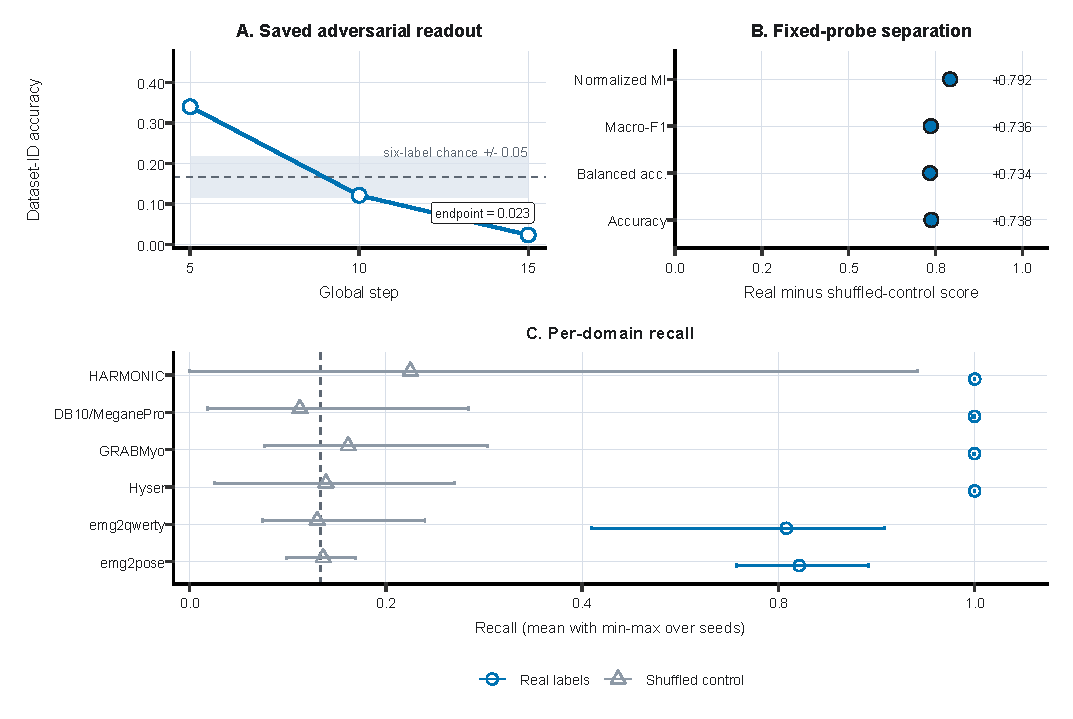
\includegraphics[width=\textwidth]{figures_compiled/fig03_domain_identifiability_audit.pdf}
\caption{Domain-identifiability audit. (A) The saved adversarial dataset-ID readout decreased from 0.3398 to 0.0234, crossing below the recorded six-label uniform reference, although the logged mini-batch rows contained only three active domains and lacked prediction-level diagnostics. (B) Independent post-freeze fixed-embedding probes across all six packaged labels recovered package/source identity with mean balanced accuracy near 0.923, while shuffled-label controls remained near the six-class reference. (C) Per-domain recall shows high recoverability for the four primary package labels and lower, partially confused recoverability for the limited emg2pose and emg2qwerty indexed subsets.}
\label{fig:domainidentifiability}
\end{figure*}

\subsection{The Audited Hyser--GRABMyo Supervised Transfer Comparison Was Not Evaluable Under the Frozen-Package Ontology Gate}
The most important boundary condition was methodological rather than merely numerical. As summarized in Table~\ref{tab:ontologygate}, the supervised transfer intersection test for Hyser$\leftrightarrow$GRABMyo reported \texttt{fail\_closed} with zero accepted classes. This is a frozen-package ontology result, not proof that the original provider datasets are intrinsically unmappable. Cross-dataset EMG studies can otherwise report invalid supervised comparisons across label spaces that are only superficially similar or incompletely documented. In contrast, the present package explicitly withheld a supervised transfer number when provider-backed one-to-one control-intent semantics could not be recovered. The source package includes the rule ledger, class dictionary, candidate mappings, and gate decisions used for this check.

The Hyser--GRABMyo supervised endpoint was withheld by a rule-based fail-closed ontology gate. Hyser contributed 34 processed manipulation codes, but the frozen package exposed them as unresolved integer labels rather than provider-backed control-intent names. GRABMyo contributed 17 processed gesture codes. Broad semantic similarity, limb-segment overlap, or ambiguous wrist/finger labels were not accepted as sufficient evidence of one-to-one control-intent equivalence. The accepted cross-dataset class intersection was therefore empty. This result sets a clear boundary on what the manuscript can claim: the fail-closed result should not be interpreted as 0\% transfer accuracy; it means the supervised cross-dataset endpoint was not validly defined under the frozen-package ontology gate. Task-valid supervised transfer remains unresolved under heterogeneous public corpora, and in some settings, the evaluation itself is not well-posed. That distinction matters because deployment-relevant robustness claims must be built on valid endpoints, not on forced comparisons across incompatible task definitions.

\begin{table*}[t]
\caption{Ontology-Gated Supervised Transfer Eligibility}
\label{tab:ontologygate}
\centering
\footnotesize
\begin{tabularx}{\textwidth}{@{}p{1.55cm}p{2.35cm}p{2.35cm}p{2.35cm}p{2.65cm}p{2.05cm}@{}}
\toprule
Dataset & Label source & Label granularity & Examples in frozen package & Accepted high-level mapping & Shared classes with paired dataset \\
\midrule
Hyser & Native Hyser manipulation annotations & 34 processed labels; codes 0--33 & Frozen package exposed unresolved integer labels; semantic control-intent names were not provider-backed in the frozen mapping file & Same-dataset identity only; no cross-dataset mapping accepted & 0; fail-closed, not evaluable \\
GRABMyo & Native GRABMyo gesture annotations & 17 processed labels; codes 0--16 & Frozen package exposed gesture-code labels; broad similarities were excluded without provider-backed one-to-one equivalence & Same-dataset identity only; no cross-dataset mapping accepted & 0; fail-closed, not evaluable \\
\bottomrule
\end{tabularx}
\vspace{0.6em}
\parbox{\textwidth}{\footnotesize\raggedright The zero intersection was not treated as a simple string-matching failure. Shared classes were accepted only under strict control-intent equivalence; ambiguous, unresolved, broad-family, or many-to-one mappings were rejected rather than converted into a supervised accuracy. The staged source-data supplement includes same-dataset identity positive controls plus symmetric Hyser$\rightarrow$GRABMyo and GRABMyo$\rightarrow$Hyser fail-closed gate decisions. No independent annotator-agreement claim is made for this frozen-package ontology gate.}
\end{table*}

\subsection{Task-Valid Downstream Screens Did Not Support a Positive Pretrained-Feature Claim}
To address whether a valid downstream endpoint could support a stronger claim, we ran same-dataset and held-out-subject screens using the frozen encoder and raw-window banks for GRABMyo and Hyser. These screens intentionally avoided Hyser--GRABMyo supervised transfer and instead asked whether pretrained features added value on task-valid within-dataset session or subject shifts.

The same-subject cross-session screen used all available processed windows in the processed raw-window package (120{,}000 embedded rows), 43 GRABMyo subjects, 20 Hyser subjects, and 10 random seeds. For normalized area under the balanced-accuracy learning curve over 1, 2, 5, and 10 target calibration windows per class, raw statistics plus pretrained features underperformed raw statistics alone by an equal-dataset mean of $-0.0622$ in the staged source table. Effects were dataset-heterogeneous: GRABMyo was negative ($-0.1743$; subject win rate 0.0), whereas Hyser was positive but smaller (+0.0499; subject win rate 0.95). The pretrained encoder did outperform a scratch encoder (+0.0641), which supports that the representation contains learned signal, but this was only a sanity check and not evidence that the encoder improves over a strong raw-statistics baseline.

A frequency-domain ridge comparator using per-channel log-bandpower, spectral-centroid, and spectral-entropy features from the same raw-window bank and the same 10-seed source-plus-calibration protocol did not reverse the conclusion. Frequency features alone were close to but still below raw statistics on the equal-dataset AULC endpoint ($-0.0043$), raw statistics plus frequency features were lower than raw statistics alone ($-0.0270$), and raw statistics plus pretrained features remained below raw statistics plus frequency features ($-0.0352$). The pattern was dataset-heterogeneous, with frequency features helping Hyser but not GRABMyo. Thus, adding a conventional frequency-domain comparator strengthened the claim boundary rather than creating a positive calibration-efficiency result.

The stricter held-out-subject few-shot screen evaluated 63 held-out subjects (43 GRABMyo, 20 Hyser), 10 seeds, trial-blocked calibration and test splits, and the normalized balanced-accuracy AULC over 1, 2, 5, and 10 calibration windows per class. It produced a useful positive control for the benchmark but not a positive claim for the pretrained representation. Raw statistics plus classical signal features improved over raw statistics alone by an equal-dataset mean of +0.0837 (subject-clustered 95\% confidence interval +0.0755 to +0.0919; one-sided subject sign-flip $p=0.0005$; subject win rate 1.0), with positive effects for both GRABMyo (+0.0945) and Hyser (+0.0728). By contrast, raw statistics plus pretrained features underperformed raw statistics alone ($-0.0457$; 95\% confidence interval $-0.0497$ to $-0.0417$; $p=1.0$ for a positive effect), with a negative GRABMyo effect ($-0.1104$) and a smaller positive Hyser effect (+0.0189). Raw statistics plus pretrained features also underperformed raw statistics plus classical signal features ($-0.1294$). Adding pretrained features on top of the classical signal baseline yielded only a small heterogeneous mean change (+0.0060; 95\% confidence interval +0.0033 to +0.0088), with GRABMyo positive (+0.0540) but Hyser negative ($-0.0419$), and did not pass the prespecified positive-claim gate because the effect was below the 0.02 threshold, dataset-heterogeneous, and not significant by the subject sign-flip criterion ($p=0.1624$). Fig.~\ref{fig:downstreamgates} visualizes these downstream gate outcomes.

The five-seed post-freeze confirmation downstream screen was also negative or mixed for a pretrained-feature claim. Across source-plus-calibration balanced-accuracy comparisons over both datasets and calibration budgets, pretrained features underperformed raw statistics on average ($-0.01437$), exceeded scratch encoders only slightly (+0.00281), and adding pretrained embeddings to raw statistics was essentially neutral overall ($-0.00042$). The combined raw-plus-pretrained effect was dataset-heterogeneous, negative for GRABMyo ($-0.00902$) and positive for Hyser (+0.00818). Because the overall effect was nonpositive and dataset effects were heterogeneous, this screen supports only a claim-boundary statement, not a reduced-calibration or pretrained-feature-superiority claim.

\begin{table*}[t]
\caption{Task-Valid Downstream Screens Used as Claim-Inclusion Gates}
\label{tab:downstreamscreens}
\centering
\footnotesize
\begin{tabularx}{\textwidth}{@{}p{2.5cm}p{3.25cm}p{4.2cm}p{2.1cm}Y@{}}
\toprule
Screen & Primary comparison & Equal-dataset effect and interval & Gate result & Interpretation \\
\midrule
Same-subject cross-session & Raw statistics + pretrained features vs. raw statistics & $-0.0622$ AULC; overall win rate 0.302 & Fail & No reduced-calibration claim over raw statistics \\
Same-subject frequency comparator & Raw + pretrained vs. raw + frequency & $-0.0352$ AULC & Fail & Conventional frequency features did not rescue a pretrained-feature advantage \\
Held-out-subject few-shot & Raw + classical signal features vs. raw statistics & +0.0837 AULC; 95\% CI +0.0755 to +0.0919 & Pass control & Benchmark detected useful task-valid signal \\
Held-out-subject few-shot & Raw + pretrained features vs. raw statistics & $-0.0457$ AULC; 95\% CI $-0.0497$ to $-0.0417$ & Fail & Pretrained features did not beat raw statistics \\
Held-out-subject few-shot & Classical + pretrained vs. classical & +0.0060 AULC; 95\% CI +0.0033 to +0.0088 & Fail & Below threshold, dataset-heterogeneous, and sign-flip $p=0.1624$ \\
Five-encoder post-freeze confirmation screen & Raw + pretrained vs. raw & $-0.00042$ balanced accuracy overall; GRABMyo $-0.00902$, Hyser +0.00818 & Fail & Near-null overall and heterogeneous across datasets \\
\bottomrule
\end{tabularx}
\end{table*}

\begin{figure*}[t]
\centering
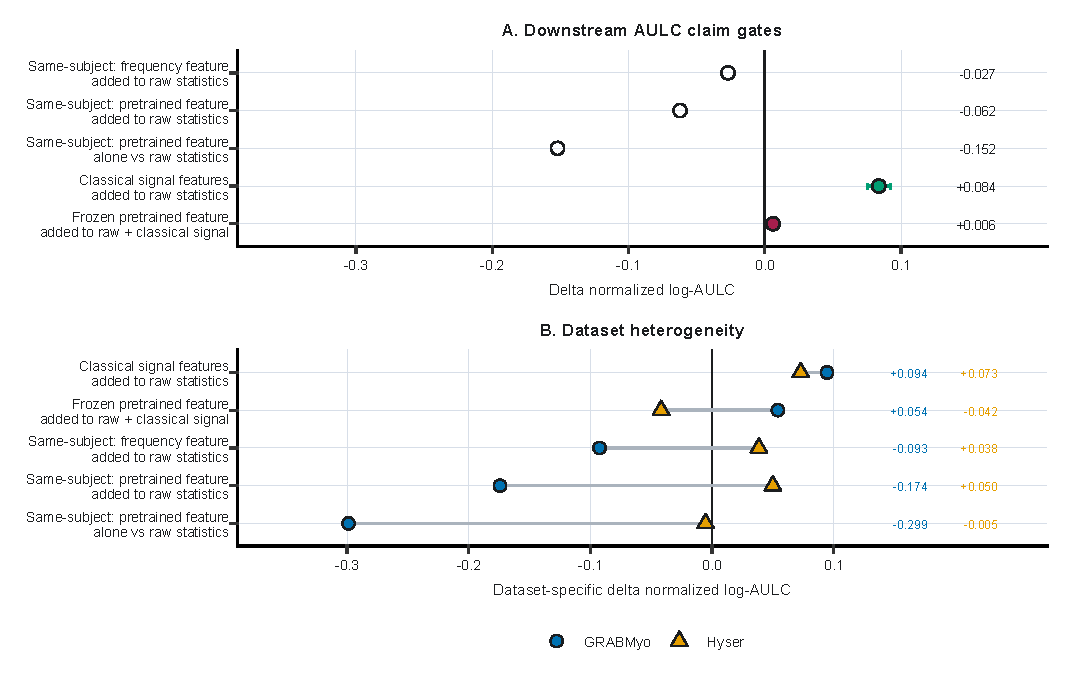
\includegraphics[width=\textwidth]{figures_compiled/fig04_downstream_claim_gates.pdf}
\caption{Downstream claim gates. (A) Task-valid calibration screens did not support a pretrained-feature-superiority claim over raw or classical signal-feature baselines, although classical features provided a positive-control improvement over raw statistics. (B) Dataset-stratified effects show why the strongest safe interpretation is a failed pretrained-superiority gate rather than reduced recalibration burden.}
\label{fig:downstreamgates}
\end{figure*}

Therefore, the downstream screens strengthened the manuscript by providing task-valid comparators, but they did not justify a claim that the frozen pretrained representation reduces calibration burden, improves over raw statistics, or improves over classical signal features.

\subsection{Descriptive Proxy Analyses Did Not Override Claim Gates}
Frozen-grid size and objective summaries are included in the supplementary material because they are descriptive rather than claim-bearing. The log-log fits of frozen-grid proxy error against tokens-seen proxy and parameter count had exponents near $\alpha\approx0.28$, and the selected composite run had lower proxy error (0.4427) than available VICReg-only, DANN-only, and CORAL-only ledger runs. These summaries help document the frozen package, but they do not establish a scaling law, causal objective superiority, ontology-valid supervised transfer, or deployment-relevant robustness. They were therefore not allowed to override the domain-ID, ontology, or downstream claim gates.

\subsection{Audit Integrity Supported Result Credibility}
The audit suite reported zero subject overlap between train and test, zero forbidden feature tokens, permutation tests below collapse thresholds, and near-machine-precision recomputation consistency. In the finalized bundle, the packaged artifact archives were both present and passed completeness checks. These signals raised confidence that the observed behaviors were not artifacts of leakage, index corruption, or undocumented reprocessing.

For a field in which impressive cross-domain claims are often difficult to verify independently, this audit layer is part of the contribution. The manuscript is therefore not only a representation-learning paper; it is also a statement about the level of artifact discipline that cross-domain EMG studies should report before robustness claims are treated as independently auditable.

\section{Discussion}
\subsection{Supported Claims for Wearable EMG Informatics}
The practical message for wearable EMG is not that the audited encoder is ready for prosthetic or rehabilitation deployment. It is that cross-domain evidence should be staged. In this package, multi-domain self-supervision produced a small positive unwhitened alignment shift, showed a small decrease in whitened alignment, and a dataset-identification endpoint that failed near-reference calibration; the five-encoder fixed-embedding probe then showed that package/source identity remained highly recoverable. These findings are useful as upstream feature-geometry and audit evidence, but they stop short of demonstrating a deployable control representation, because task-valid transfer also requires a defensible shared label ontology and downstream evidence tied to control quality, recalibration burden, or user-facing reliability.

The central result is negative in the direction that matters for deployment-facing claims: the encoders can contain learned signal while still preserving package/source identity, and their pretrained features do not establish superiority over simple raw-statistical or classical signal baselines. This does not make the audit uninformative; it is precisely the failure mode the claim-gated framework is meant to expose. The manuscript should therefore be read as evidence for stronger claim control in cross-domain EMG representation studies, not as evidence that the audited encoder learned a domain-invariant or deployment-ready control representation.

The audited package increased off-diagonal CKA and the selected composite run had lower observed proxy error than the single-component ablations, but the auxiliary alignment endpoints were mixed: wCKA slightly decreased and cluster top-1 remained inconclusive under the pair-level interval. These patterns are inconsistent with a single obvious collapse explanation in the saved summaries, but they do not rule out partial collapse, domain-label permutation, or adversarial-readout instability; nor do they establish semantic transfer. At the same time, the nominal adversarial dataset-ID readout overshot below the recorded reference, independent probes recovered package/source identity with high balanced accuracy, and the package withheld supervised transfer when class semantics were not aligned. The learned geometry, therefore, provided limited label-agnostic evidence without becoming a universally transferable semantic task space.

CKA and wCKA should therefore be read as complementary diagnostics rather than interchangeable confirmations. Unwhitened CKA can increase when broad covariance or anisotropic variance structure becomes more similar across domains, whereas wCKA asks whether alignment remains after within-dataset covariance structure is removed. The observed split is mixed evidence: it supports a small unwhitened geometry shift but not a robust whitening-invariant alignment claim.

The downstream screens reinforce that boundary rather than weakening it. The same-subject session-shift screen showed that pretrained features were better than scratch features, but they did not improve over raw time-domain statistics in the prespecified primary comparison, nor did they outperform the added frequency-domain comparator. The held-out-subject few-shot screen added a stronger task-valid benchmark and showed that classical signal features can improve over raw statistics, but the frozen pretrained representation did not beat raw statistics or the classical signal baseline by the prespecified gate. The five-encoder post-freeze confirmation was also null or negative for pretrained-feature superiority: pretrained-only features underperformed raw statistics overall, and adding pretrained embeddings to raw statistics was essentially neutral with opposite signs in GRABMyo and Hyser. This distinction is important for interpretation: representation learning can be nontrivial and still fail to justify deployment-facing claims about reduced recalibration burden or task-valid transfer.

The following claims are therefore not supported by this audit: calibrated domain invariance, whitening-invariant cross-domain alignment, supervised Hyser--GRABMyo transfer, calibration-free rehabilitation control, reduced recalibration burden, EMGBench-level generalization, online prosthetic-control readiness, or clinical deployment readiness. These negative boundaries are part of the contribution because they prevent a frozen representation package from being overinterpreted.

\subsection{Label Mismatch Is a Structural Barrier}
The fail-closed Hyser$\leftrightarrow$GRABMyo result is central. Hyser is an HD-sEMG neural-interface dataset with fine-grained dexterous manipulation structure \cite{jiang2021hyser}, whereas GRABMyo emphasizes multi-day sEMG gesture recognition and biometrics from forearm and wrist placements \cite{pradhan2022grabmyo}. These are both valuable EMG resources, but they do not define a ready-made, shared supervised ontology. Under these conditions, reporting a transfer number would be easier to summarize but less methodologically defensible than an explicit fail-closed outcome.

For prosthetic-control and rehabilitation-interface studies, this fail-closed behavior is best treated as a conservative design criterion rather than a missing result. A transfer score is only actionable when the source and target tasks describe the same control intent at a control-intent level relevant to the benchmark objective. Otherwise, a high number may reflect an artificial benchmark construction rather than evidence that a user could rely on the interface with less calibration or greater consistency.

This observation also clarifies how recent reusable-encoder language should be interpreted. Large and diverse public corpora such as emg2qwerty and emg2pose make representation reuse a reasonable research objective \cite{sivakumar2024emg2qwerty,salter2024emg2pose}. But reusable pretraining and valid supervised transfer are not the same claim. In the present package, the data support only preliminary upstream representation-level evidence; they do not support a claim that task-valid supervised transfer across arbitrary public EMG datasets has already been solved.

\subsection{Why the Overshoot Matters}
The below-reference dataset-ID endpoint is not merely a numerical detail. It changes the interpretation of the invariance result. If the discriminator had converged to chance, one could argue that the encoder learned features that suppress domain identity while retaining task-relevant structure. Falling far below the recorded reference introduces ambiguity, and the five-encoder fixed-embedding probes convert that ambiguity into a failed invariance claim for the probed package/source embeddings: package/source identity remained highly recoverable across six packaged labels. The most defensible interpretation is therefore not calibrated invariance, but a diagnostically incomplete adversarial-readout endpoint that requires independent diagnostics before any invariance claim is accepted.

This nuance is especially relevant when these methods are proposed for wearable health or rehabilitation systems. A representation with low nominal domain-ID accuracy is not automatically a clinically or operationally robust one. In sensor-informatics terms, \emph{robustness} requires more than reducing one nuisance readout; it requires preserving the right information under the shifts that affect control quality, reliability, and recalibration burden.

What would have passed? A calibrated domain-invariance claim would have required a held-out, balanced all-six-packaged-domain diagnostic with nondegenerate prediction marginals, low mutual information, low optimal-relabel recoverability, and no contradictory fixed-probe recoverability. A supervised-transfer claim would have required a documented one-to-one control-intent ontology. A reduced-calibration or pretrained-feature-superiority claim would have required positive, dataset-consistent downstream gains over raw and classical signal-feature baselines under the prespecified gates. Deployment-facing prosthetic-control claims would require online control, reliability, workload, and user-facing performance endpoints, which this audit did not test.

\subsection{Relationship to Recent Calibration-Free and Large-Corpus EMG Work}
Recent EMG studies have used self-supervised learning and/or domain alignment to improve cross-subject robustness \cite{yang2025calibrationfree,raghu2025vicregemg}, and benchmark-scale public datasets now enable broader evaluation of representation reuse \cite{sivakumar2024emg2qwerty,salter2024emg2pose}. Foundation-model-oriented preprints such as EMGNet further push the field toward larger, more heterogeneous pretraining corpora and cross-device evaluation \cite{kurbis2025emgnet}. This study does not evaluate these foundation-model claims directly. It asks which reuse claims remain valid after ontology checks, domain-identifiability diagnostics, downstream baseline gates, and audit gates.

The present paper therefore complements, rather than contradicts, the recent literature. It separates evidence that is present in this package (a small unwhitened alignment shift, lower composite-run proxy error within a frozen grid, rigorous artifact completeness, pretrained features that nominally outperformed scratch features in a sensitivity screen, and a positive classical signal-feature control in a held-out-subject few-shot benchmark) from claims that remain premature (calibrated domain invariance, supervised transfer across heterogeneous public corpora with mismatched ontologies, pretrained-feature superiority over raw or classical signal baselines, or calibration-burden reduction). The downstream result rejects a positive claim for this frozen encoder under these task-valid ridge-readout screens; it does not reject all possible EMG pretraining.


\subsection{Limitations}
This study has five main limitations. First, the main evaluation matrix covered four primary feature-bank domains, even though six packaged domain labels were present in the training mixture; emg2qwerty and emg2pose were limited indexed subsets, not full benchmark utilization. Second, the composite objective was evaluated through frozen artifacts. This improves reproducibility and reduces post hoc optimization, but it limits architectural introspection, makes the proxy-error size analysis descriptive, and prevents interpreting the three-size grid as a universal EMG scaling law.

Third, the uncertainty and package/source-identifiability evidence remain incomplete. The CKA/wCKA estimates are pair-balanced summaries over six unordered four-domain pairs, with direction-labeled rows retained only as sampling diagnostics, rather than participant-level or sample-weighted estimates; alternative dataset-weighting schemes were not evaluated. The study also did not run the standardized EMGBench task suite or compare against EMGBench leaderboard baselines. For package/source identification, the canonical six-label frozen summary did not expose the original adversarial-head prediction-level confusion matrix, true and predicted marginals, prediction entropy, balanced accuracy, optimal-relabel accuracy, mutual information, or readout-training traces. The five-encoder six-packaged-domain fixed probe closes the independent fixed-embedding recoverability gap for the six packaged labels, but it still does not reconstruct the original adversarial readout, does not identify whether recoverability reflects physiology, hardware, protocol, preprocessing, or package artifacts, and does not make emg2qwerty or emg2pose full benchmark evaluations. However, because package/source identity was highly recoverable across five independently trained encoders while shuffled controls were near the six-class reference, the result is sufficient to reject calibrated domain-invariance language for the audited embeddings.

Fourth, preprocessing and baseline scope were deliberately constrained. Heterogeneous inputs were standardized to 16 channels and 64-sample windows, so electrode topology, HD-sEMG grid adjacency, channel-density effects, and longer-window spectral structure may be compressed or discarded. The downstream screens used offline raw-window GRABMyo and Hyser readouts with ridge classifiers and added classical log-bandpower, shrinkage log-Euclidean covariance, and short-time-Fourier summary features, but they did not include neural spectrogram, continuous-wavelet-transform scalogram, topology-preserving raw-tensor, SEA++-style sensor alignment, full Riemannian tangent-space/minimum-distance-to-mean classifiers, or standardized EMGBench task-suite baselines. Fifth, the manuscript is bounded to offline retrospective public-data evaluation. It does not establish clinical readiness, online shared-autonomy benefit, patient-facing usability, long-term deployment outcomes, ontological design, or fairness under demographic distribution shift. A recently released dataset with explicit demographic and physiological metadata makes these questions more testable \cite{gowda2025demographicsemg}, but it was outside the frozen package evaluated here.

\subsection{Practical Implication for Sensor Informatics}
A conservative reporting implication for wearable sensor informatics is to report cross-domain evidence in layers. First, domain-identifiability analysis asks whether nuisance information, such as dataset or package/source identity, has been reduced, and whether that reduction is calibrated rather than below-reference and ambiguous. Second, label-agnostic compatibility asks whether independently collected EMG datasets occupy a more compatible feature geometry. Third, task-valid transfer asks whether a shared supervised endpoint is semantically justified. Prosthetic-control and rehabilitation-interface claims require the third layer and will eventually require online evidence about workload \cite{park2024workload}, control reliability, usability, and recalibration burden. The present results partially support upstream representation-level evidence but deliberately withhold task-valid transfer when the ontology check fails. This separation makes the findings useful for audit-oriented EMG research while preserving the boundary between feature-geometry evidence and task-valid transfer evidence.

\section{Conclusion}
We presented an audit-gated claim-control framework for cross-domain self-supervised EMG representation learning using a frozen public-data artifact package. The strongest defensible result is not that the encoder improves prosthetic-control transfer, reduces recalibration burden, or learns domain-invariant features; it is that a claim ledger can prevent these claims when the evidence is incomplete or contradictory. In this package, unwhitened CKA increased slightly under unordered-pair sensitivity while wCKA decreased; the original six-label adversarial package/source-ID endpoint was below reference but diagnostically incomplete; independent fixed probes recovered package/source identity; Hyser--GRABMyo supervised transfer was not evaluable because provider-backed one-to-one control-intent semantics were absent from the frozen package; and downstream session-shift and held-out-subject screens did not establish pretrained-feature superiority over raw or classical features. A classical signal-feature baseline improved held-out-subject performance, confirming that the downstream benchmark could detect useful task-valid signal. For wearable EMG, deployment-facing claims should therefore require ontology-aware tasks, calibrated domain-recoverability diagnostics, strong baselines, and evaluation endpoints linked to control reliability, recalibration burden, and user-facing performance under realistic acquisition shift.
\section*{Ethics and Data Governance}
This retrospective secondary analysis used only previously released third-party datasets and derived public-data artifacts. No new participants were recruited, no intervention was performed, and no new identifiable private health information was collected by the authors. Ethics approval and consent procedures for the source datasets are described in the original dataset publications. Raw third-party EMG data are not redistributed in this manuscript package; users must obtain source datasets under the original provider access terms.

\section*{Data and Code Availability}
All source datasets used in this study are available from their original repositories, including HARMONIC \cite{newman2022harmonic}, NinaPro DB10 and MeganePro \cite{atzori2014ninapro,giordaniello2017meganepro}, GRABMyo version 1.0.2 \cite{pradhan2022grabmyo}, Hyser version 1.0.0 \cite{jiang2021hyser}, emg2qwerty \cite{sivakumar2024emg2qwerty}, and emg2pose \cite{salter2024emg2pose}, subject to the access terms of the original dataset providers. Raw third-party data are not redistributed. For peer review, the anonymized source package supplied through the review system includes the LaTeX sources, compiled PDFs, vector figures, figure-building script, manuscript-ready source tables, package manifest, and checksum ledger needed to trace the reported values. Public repository and archive identifiers are withheld from this review copy and can be restored in the accepted version.

\section*{Conflict of Interest}
The authors declare no conflict of interest.

\section*{Acknowledgment}
The authors thank the creators and maintainers of the public EMG datasets and benchmarks that made this work possible. AI-assisted tools, including OpenAI ChatGPT and OpenAI Codex, were used for language polishing, consistency checking, and source-package verification support in the manuscript, supplementary material, and package documentation. They were not used to generate datasets, statistical results, figures, references, or scientific claims. All analyses, interpretations, claims, and final submitted text were reviewed and approved by the authors, who take full responsibility for the work.

\bibliographystyle{IEEEtran}
\bibliography{refs}

\end{document}
